\documentclass[withoutpreface,bwprint]{cumcmthesis}

\usepackage{float}
\usepackage{url}
\usepackage{booktabs}  
\usepackage{threeparttable} 
\usepackage{parskip}
\usepackage{subfigure}
\usepackage{epstopdf}
\usepackage{indentfirst}
\usepackage{graphics}
\setlength{\parindent}{1.5em}
\begin{document}
\section{实验目的}
实现一个K-Means算法和混合高斯模型,并且用EM算法估计模型中的参数。

\section{实验要求及实验环境}
\subsection{实验要求}
\begin{enumerate}
\setlength{\itemindent}{1.5em}
\item 用高斯分布产生k个高斯分布的数据(不同的均值和方差),其中参数自定;
\item 使用K-Means聚类,测试效果;
\item 用EM算法估计参数,观察每次迭代后似然值的变化,考察EM算法是否得到正确的结果;
\item 在UCI网站上找一组数据集观测效果。
\end{enumerate}

\subsection{实验环境}
\begin{itemize}
\setlength{\itemindent}{1.5em}
\item 硬件:Intel i5-8265U、512G SSD、8G RAM;
\item 系统:Windows 11;
\item IDE:Pycharm。
\end{itemize}

\section{设计思想}
\subsection{K-Means原理}
给定训练样本$\boldsymbol{X}=\{\boldsymbol{x_{1}},\boldsymbol{x_{2}},\cdots,\boldsymbol{x_{n}}\}$和划分聚类的数量$k$,给定一个簇划分$C=C_{1},C_{2},\cdots,C_{k}$,使得该划分的平方误差$E$最小化,即使下式取最小值:
\begin{equation*}
E=\sum_{i=1}^{k}\sum_{\boldsymbol{x}\in C_{i}}\left \| \boldsymbol{x}-\boldsymbol{\mu_{i}} \right \|
\end{equation*}

其中,$\boldsymbol{\mu_{i}}=\frac{1}{C_{i}}\sum_{\boldsymbol{x}\in C_{i}}\boldsymbol{x}$,为簇$C_{i}$的均值向量。$E$刻画了簇内样本围绕簇的均值向量的紧密程度,$E$越小簇内样本的相似度相似度越高。

\subsection{GMM原理}
多元高斯分布生成的$m$维随机变量$\boldsymbol{x}$的密度函数为
\begin{equation*}
p(\boldsymbol{x}|\boldsymbol{\mu},\boldsymbol{\Sigma})=\frac{1}{(2\pi)^{\frac{m}{2}}\left|\boldsymbol{\Sigma}\right|^{\frac{1}{2}}}\exp{(-\frac{1}{2}(\boldsymbol{x}-\boldsymbol{\mu})^{T}\boldsymbol{\Sigma}^{-1}(\boldsymbol{x}-\boldsymbol{\mu}))}
\end{equation*}

其中$\boldsymbol{\mu}$为$m$维的均值向量,$\boldsymbol{\Sigma}$为$m\times m$的协方差矩阵。

给定训练样本$\boldsymbol{X}=\{\boldsymbol{x_{1}},\boldsymbol{x_{2}},\cdots,\boldsymbol{x_{n}}\}$,他是一个$n\times m$的矩阵,$n$为样本数量,$m$为单个样本的维度。我们可以认为此样本集是由多个维度为$m$的多元高斯分布混合而成,即:
\begin{equation*}
p(\boldsymbol{x_{j}})=\sum_{i=1}^{k}\pi_{i} p(\boldsymbol{x_{j}}|\boldsymbol{\mu_{i}},\boldsymbol{\Sigma_{i}})
\end{equation*}

其中$\boldsymbol{\mu_{i}}$,$\boldsymbol{\Sigma_{i}}$是第$i$个高斯分布的均值和协方差矩阵,$\pi_{i}$为相应的混合系数,满足$\sum_{i=1}^{k}\pi_{i}=1$。

要求解$\pi$、$\boldsymbol{\mu}$、$\boldsymbol{\Sigma}$可以使用极大似然来估计样本集$\boldsymbol{X}$,有:
\begin{equation*}
\ln p(\boldsymbol{X}|\pi,\boldsymbol{\mu},\boldsymbol{\Sigma})=\ln \prod_{j=1}^{n} p(\boldsymbol{x_{j}})=\sum_{j=1}^{n}\ln \sum_{i=1}^{k}\pi_{i}p(\boldsymbol{x_{i}}|\boldsymbol{\mu_{i}},\boldsymbol{\Sigma_{i}})
\end{equation*}

要使上式最大化,分别对$\pi_{i}$、$\mu_{i}$、$\Sigma_{i}$求偏导
\begin{equation*}
\frac{\partial{\ln p(\boldsymbol{X}|\pi,\boldsymbol{\mu},\boldsymbol{\Sigma})}}{\partial{\boldsymbol{\pi_{i}}}}=0
\end{equation*}
\begin{equation*}
\frac{\partial{\ln p(\boldsymbol{X}|\pi,\boldsymbol{\mu},\boldsymbol{\Sigma})}}{\partial{\boldsymbol{\mu_{i}}}}=0
\end{equation*}
\begin{equation*}
\frac{\partial{\ln p(\boldsymbol{X}|\pi,\boldsymbol{\mu},\boldsymbol{\Sigma})}}{\partial{\boldsymbol{\Sigma_{i}}}}=0
\end{equation*}

解得
\begin{equation}
\gamma(z_{ji})=\cfrac{p(z_{i}=1|\boldsymbol{x_{j}})}{\sum_{i=1}^{k}p(z_{i}=1|\boldsymbol{x_{j}})}=\cfrac{\pi_{i}p(\boldsymbol{x_{j}}|\boldsymbol{\mu_{i}},\boldsymbol{\Sigma_{i}})}{\sum_{l=1}^{k}\pi_{l}p(\boldsymbol{x_{j}}|\boldsymbol{\mu_{l}},\boldsymbol{\Sigma_{l}})}
\end{equation}

\begin{equation}
\pi_{i}=\frac{\sum_{j=1}^{n}\gamma(z_{ji})\boldsymbol{x_{j}}}{n}
\end{equation}

\begin{equation}
\mu_{i}=\frac{\sum_{j=1}^{n}\gamma(z_{ji})\boldsymbol{x_{j}}}{\sum_{j=1}^{n}\gamma(z_{ji})}
\end{equation}

\begin{equation}
\Sigma_{i}=\frac{\sum_{j=1}^{n}\gamma(z_{ji})(\boldsymbol{x_{j}}-\boldsymbol{\mu_{i}})(\boldsymbol{x_{j}}-\boldsymbol{\mu_{i}})^{T}}{\sum_{j=1}^{n}\gamma(z_{ji})}
\end{equation}

\section{算法设计}
\subsection{K-Means}
K-Means算法的步骤大致如下:
\begin{enumerate}
\item 根据输入的超参数首先初始化一些向量(可以从现有的向量中挑选),作为各簇的均值向量;
\item 首先根据输入的超参数$k$初始化一组向量作为各簇的均值向量,可以随机生成,或从数据集中随机挑选。
\item 将数据集中所有的向量划分到各个簇中,使得他们离所在簇的均值向量的距离最小;
\item 根据簇中所有的向量,求得新的均值向量。
\item 对2,3步进行一定次数的迭代。
\end{enumerate}

\subsection{GMM}
GMM算法的步骤大致如下:
\begin{enumerate}
\item 随机初始化参数$\pi_{i}$、$\mu_{i}$、$\Sigma_{i}$,$i \in \{1,2,\cdots,k\}$;
\item 根据式(1)初始化每个样本由各个混合高斯分步生成后的后验概率;
\item 根据式(2)、(3)、(4)更新$\pi_{i}$、$\mu_{i}$、$\Sigma_{i}$;
\item 对2,3步进行一定次数的迭代。
\end{enumerate}

\section{实验结果与分析}
\subsection{混合高斯模型}
可以看到此时在迭代次数较小的情况下,分类效果仍然比较好。

\begin{figure}[H]
    \centering
    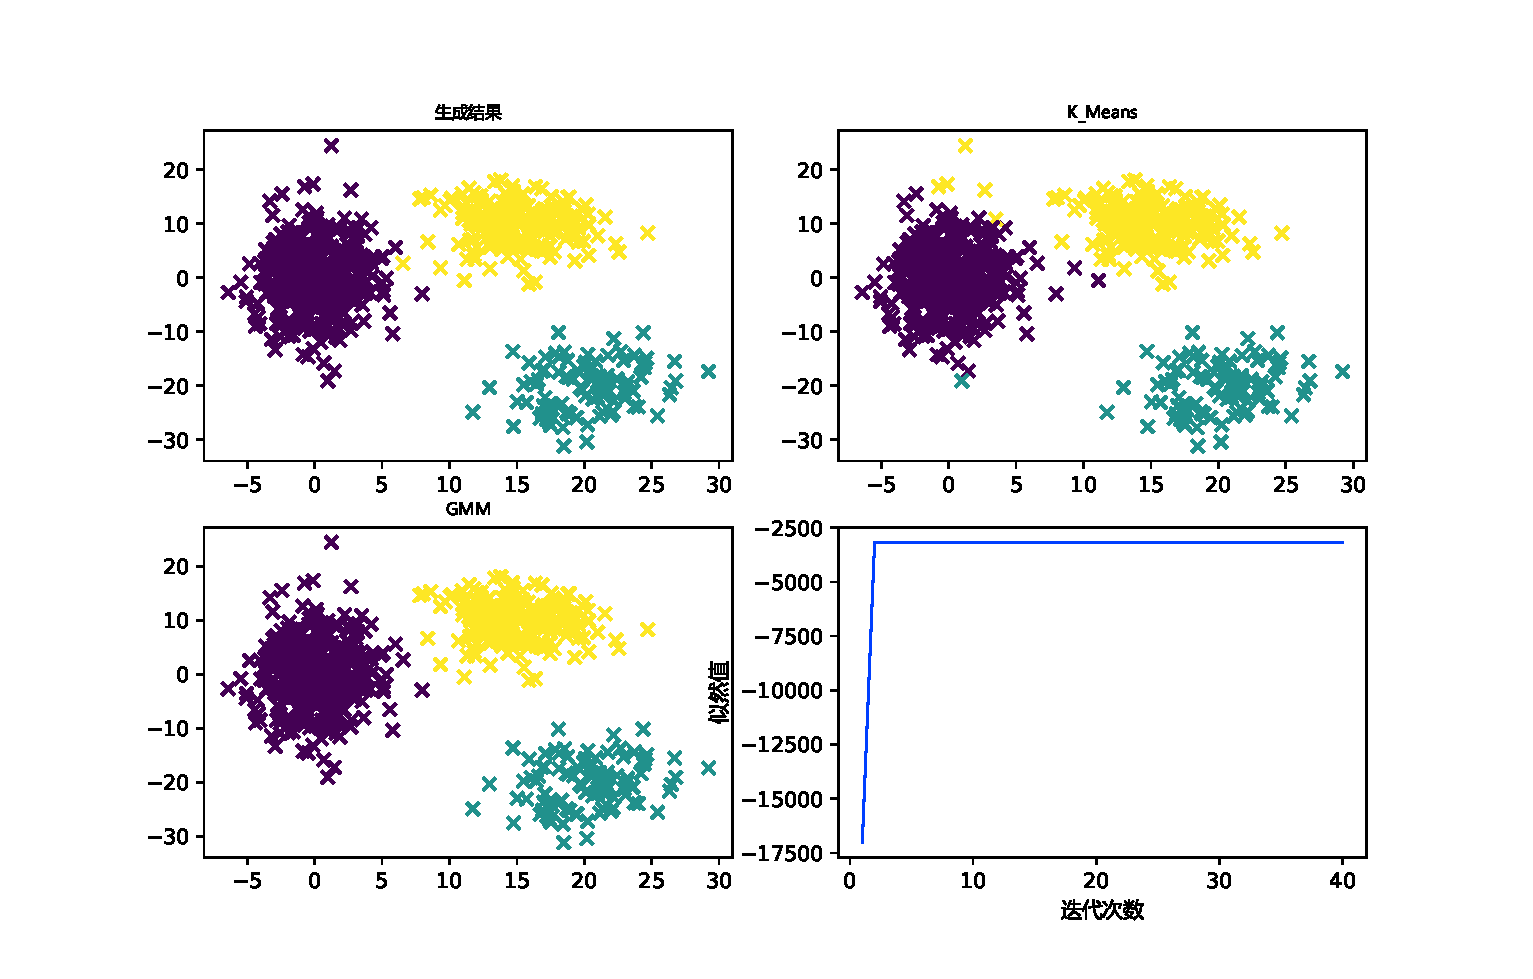
\includegraphics[width=0.8\textwidth]{Figure_1}
    \caption{混合高斯模型效果}
    \label{图1}
\end{figure}

此时K\_Means、GM两方法均迭代40次,最后准确率分别为98.71\%、99.86\%。

\subsection{iris数据集}

\begin{figure}[H]
    \centering
    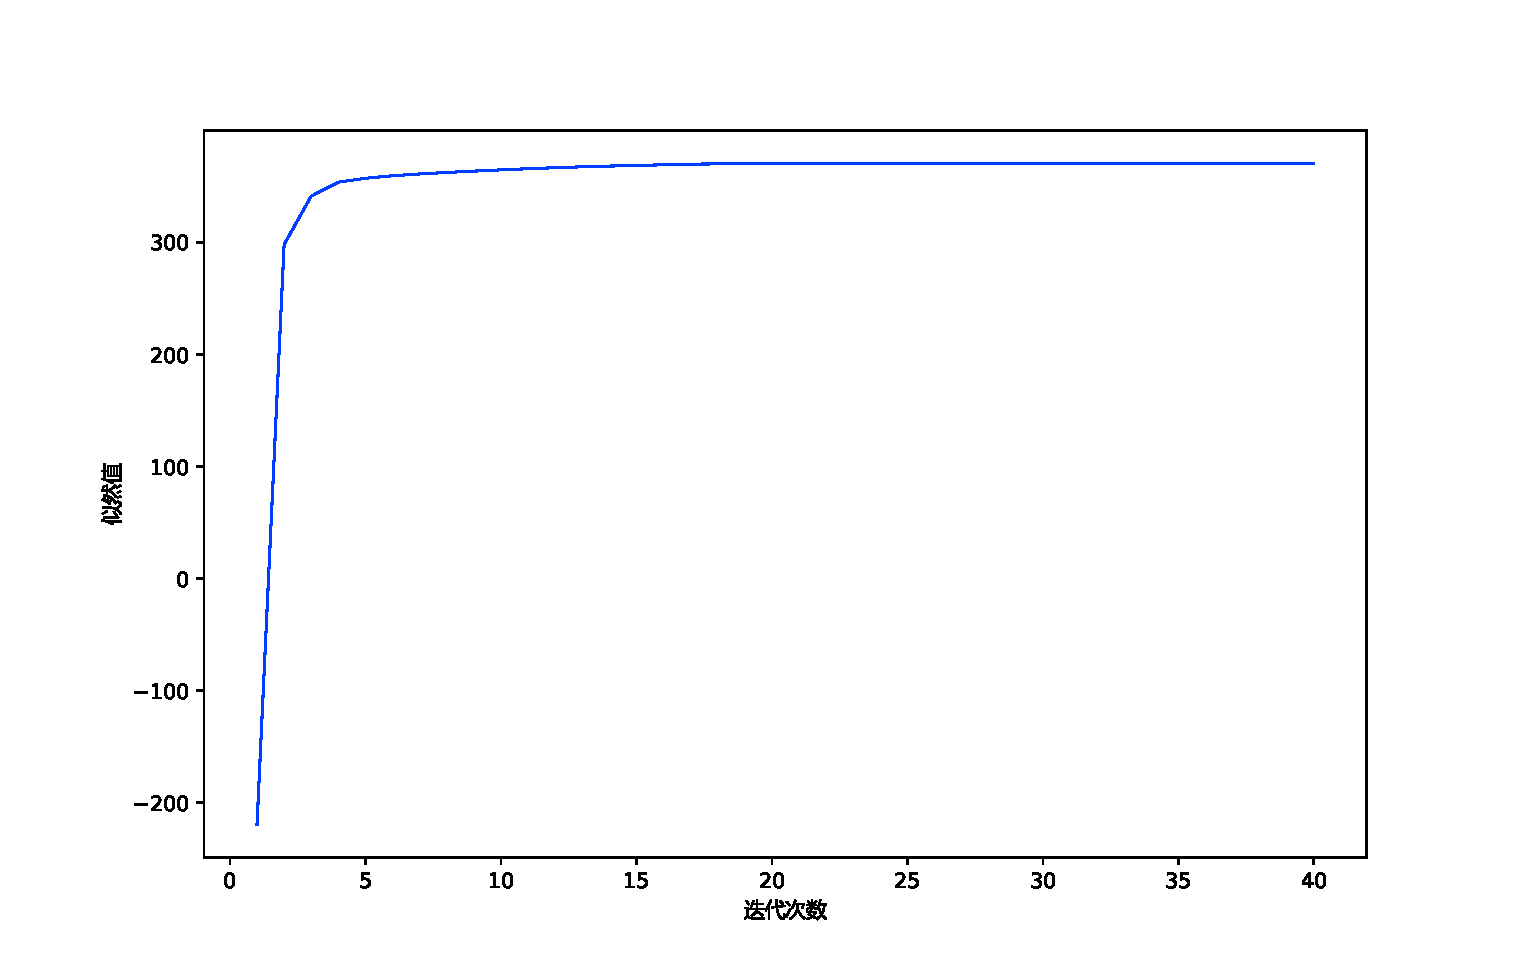
\includegraphics[width=0.8\textwidth]{Figure_2}
    \caption{iris数据集}
    \label{图2}
\end{figure}

此时K\_Means、GM两方法均迭代40次,最后准确率分别为89.33\%、96.67\%。


\section{结论}
K-Means实际上假设数据式呈球状分布,假设使用的欧式距离来衡量样本与各个簇中心的相似度(假设数据的各个维度对于相似度计算的作用是相同的),它的簇中心初始化对于最终的结果有很大的影响,如果选择不好初始的簇中心值容易使之陷入局部最优解;与之相比GMM使用更加一般的数据表示即高斯分布,GMM使用EM算法进行迭代优化,因为其涉及到隐变量的问题,没有之前的完全数据,而是在不完全数据上进行。

K-Means其实就是一种特殊的高斯混合模型,假设每种类在样本中出现的概率相等均为$\frac{1}{k}$,而且假设高斯模型中的每个变量之间是独立的,即变量间的协方差矩阵是对角阵,这样我们可以直接用欧氏距离作为K-Means的协方差去衡量相似性;K-Means对响应度也做了简化,每个样本只属于一个类,即每个样本属于某个类响应度为1,对于不属于的类响应度设为0,算是对GMM的一种简化。而在高斯混合模型中,每个类的数据出现在样本中的概率为,用协方差矩阵替代K-Means中的欧式距离去度量点和点之间的相似度,响应度也由离散的0,1变成了需要通过全概率公式计算的值。由于GMM不像K-Means做了很多假设,所以分类最终效果比K-Means好,但是GMM-EM算法过于细化,容易被噪声影响,所以适合对K-Means的分类结果进行进一步优化。

\newpage
\begin{appendix}
\section{主程序}
\begin{lstlisting}[language=python]
import copy
import random

import matplotlib.pyplot as plt
import pandas as pd

from graph import init_graph, draw_graph, font_title, font_label
import numpy as np

dimension_num = 0
k = 0
iteration_times_K_Means = 10
iteration_times_GMM = 10


def get_mixture_guassian(size_list, mean_list, cov_matrix_list):
    total_data = [[0.0] * dimension_num] * sum(size_list)
    temp_index = 0
    seed = []
    for i in range(k):
        temp_list = np.random.multivariate_normal(mean_list[i], cov_matrix_list[i], size_list[i])
        total_data[temp_index:temp_index + size_list[i]] = [temp.tolist() + [i] for temp in temp_list]
        seed.append(total_data[temp_index])
        temp_index += size_list[i]

    random.shuffle(total_data)
    return [data[:-1] for data in total_data], [data[-1] for data in total_data], seed


def get_iris():
    field_list = ["sepal_length", "sepal_width", "petal_length", "petal_width"]
    label_dict = {"Iris-setosa": 0, "Iris-versicolor": 1, "Iris-virginica": 2}
    raw_data = pd.read_csv("iris.data", names=field_list + ["label"], nrows=150)

    processed_data = []
    processed_data_label = []

    for i in range(len(raw_data)):
        processed_sample = []
        raw_sample = raw_data.iloc[i]

        try:
            for field in field_list:
                processed_sample.append(float(raw_sample.loc[field]))
        except KeyError:
            continue
        except ValueError:
            continue

        processed_data_label.append(label_dict[raw_sample.loc["label"]])
        processed_data.append(processed_sample)

    seed = [processed_data[0] + [0], processed_data[50] + [1], processed_data[100] + [2]]
    return processed_data, processed_data_label, seed


def K_Means(X_list, seed):
    U = np.array([temp[:-1] for temp in seed])
    label = [temp[-1] for temp in seed]
    X = np.array(X_list)
    Y = [0] * len(X_list)

    for i in range(iteration_times_K_Means):
        for j in range(len(X_list)):
            min_distance = np.dot(X[j] - U[0], X[j] - U[0])
            for m in range(k):
                temp_distance = np.dot(X[j] - U[m], X[j] - U[m])
                if temp_distance < min_distance:
                    min_distance = temp_distance
                    Y[j] = label[m]

        U = np.array([[0.0] * dimension_num] * k)
        Num = np.zeros(k)
        for j in range(len(X_list)):
            U[Y[j]] += X[j]
            Num[Y[j]] += 1

        for m in range(k):
            U[m] /= Num[m]
    return Y


def GMM(X_list, seed):
    length = len(X_list)
    U = np.array([temp[:-1] for temp in seed])
    label = [temp[-1] for temp in seed]
    X = np.array(X_list)
    Cov = [np.diag([1] * dimension_num)] * k
    P = [1 / k] * k
    result = [[1 / k] * k] * length
    likelihood_list = [0.0] * iteration_times_GMM

    for t in range(iteration_times_GMM):
        for j in range(length):
            for i in range(k):
                result[j][i] = P[i] * (1 / np.sqrt(np.linalg.det(Cov[i]))) * np.exp(
                    -0.5 * np.dot((np.dot((X[j] - U[i]).T, np.linalg.pinv(Cov[i]))), X[j] - U[i]))
            temp = sum(result[j])
            likelihood_list[t] += np.log(temp)
            result[j] = [result[j][i] / temp for i in range(k)]

        U = np.array([[0.0] * dimension_num] * k)
        for i in range(k):
            temp = sum(result[j][i] for j in range(length))
            U[i] = sum([X[j] * result[j][i] for j in range(length)]) / temp
            Cov[i] = sum([np.dot((X[j] - U[i]).reshape(dimension_num, 1), (X[j] - U[i]).reshape(1, dimension_num)) * result[j][i] for j in
                          range(length)]) / temp
            P[i] = sum([result[j][i] for j in range(length)]) / length

    Y = [result[j].index(max(result[j])) for j in range(length)]
    Y = [label[Y[j]] for j in range(length)]
    return Y, likelihood_list


def test(predict_Y_list, Y_list):
    correct_num = 0
    total_num = len(Y_list)
    for i in range(len(Y_list)):
        if predict_Y_list[i] == Y_list[i]:
            correct_num += 1
    return correct_num / total_num


def show(X_list, raw_Y_list, K_Means_Y_list, GMM_Y_list, likelihood_list):
    init_graph(plt)
    if dimension_num==2:
        total_Y_list = [raw_Y_list, K_Means_Y_list, GMM_Y_list]
        title_list = ["生成结果", "K_Means", "GMM", "似然值"]
        X_list_one = [x[0] for x in X_list]
        X_list_two = [x[1] for x in X_list]

        for i in range(3):
            plt.subplot(2, 2, i + 1)
            plt.title(title_list[i], font=font_title)
            plt.scatter(X_list_one, X_list_two, c=total_Y_list[i], marker="x")

        plt.subplot(2, 2, 4)

    plt.xlabel(fontdict=font_label, xlabel="迭代次数")
    plt.ylabel(fontdict=font_label, ylabel="似然值")
    plt.plot([i + 1 for i in range(len(likelihood_list))], likelihood_list, linewidth=1)
    draw_graph(plt)


if __name__ == '__main__':
    # size_list = [400, 100, 200]
    # mean_list = [[0, 0], [20, -20], [15, 10]]
    # cov_matrix_list = [[[5, 0.2], [0.2, 40]], [[10, 0.5], [0.5, 20]], [[10, 0.3], [0.3, 15]]]
    # k = 3
    # dimension_num = 2
    #
    # X_list, Y_list, seed = get_mixture_guassian(size_list, mean_list, cov_matrix_list)
    X_list, Y_list, seed = get_iris()
    k = 3
    dimension_num = 4

    K_Means_Y_list = K_Means(X_list, seed)
    GMM_Y_list, likelihood_list = GMM(X_list, seed)

    print("K_Means:", test(K_Means_Y_list, Y_list))
    print("GMM:", test(GMM_Y_list, Y_list))
    show(X_list, Y_list, K_Means_Y_list, GMM_Y_list,likelihood_list)

\end{lstlisting}

\section{可视化}
\begin{lstlisting}[language=python]
# 设置字体,解决中文无法识别的问题
# 图表标题
font_title = {
    'family': 'Microsoft Yahei',
    'weight': 'regular',
    'size': 8
}

# 坐标轴标题
font_label = {
    'family': 'Microsoft Yahei',
    'weight': 'regular',
    'size': 10
}

# 图例
font_legend = {
    'family': 'Microsoft Yahei',
    'weight': 'regular',
    'size': 6
}


def init_graph(plt, dpi=150, style="seaborn-bright"):
    # 设置清晰度
    plt.figure(dpi=dpi)

    # 设置样式
    plt.style.use(style)


def draw_graph(plt, save=True, filename="picture.jpg", show=True):
    # 是否保存
    if save:
        plt.savefig("./figures/" + filename)

    if show:
        plt.show()
\end{lstlisting}
\end{appendix}
\end{document}
